\chapter{Introduction}
  \section{The Inequalities of Interactivity}
    We are surrounded by products with dedicated physical interfaces, like
    steering wheels, musical instruments, and game controllers. While the advent
    of screen-based devices has led to a rise in touch, and mouse based
    applications, there are some benefits of physicality that simply do not
    translate to screens~\cite{klemmer:2006}. It is because of these benefits
    (e.g., hands-free interaction, speed, virtuosity, control) that most experts
    use dedicated physical interfaces for their crafts, rather than their screen
    counterparts.

    Because the increased presence of screen-based devices, significant advances
    has been made to streamline the creation of screen-based applications.  In
    60 years, the state-of-the-art has gone from programming computers using
    punched cards, to creating immersive virtual environments by dragging
    virtual elements and dropping them in their respective
    places~\footnote{\href{https://unity.com}{Unity}}.  Currently, you can
    create an online store without knowing anything about web
    programming~\footnote{\href{https://www.squarespace.com}{Squarespace}}, or
    creating body-based augmented reality applications using visual
    programming~\cite{Pohl:2020}.

    Contrary to this ease of crafting interactive digital experiences,
    constructing interactive physical objects remains a challenging undertaking.
    While the construction, and usage of interactive digital interactive
    experiences has been researched for over forty years~\cite{CHI:, UIST:}, no
    long-term research has explored ways to construct interactive experiences in
    the physical world. Because of this, constructing physical interactive
    experiences still require significant domain knowledge, and remains out of
    reach for other-domain experts. Although existing research has explored
    electronic toolkits to lower the threshold of making physical, interactive
    devices~\cite{Greenberg:2001, Arduino:}, these require the assembly of
    electronic sensors, actuators and physical parts to construct an interactive
    device.

    While the process of assembling circuits and printed parts may seem
    straightforward to some, this is an intricate process, and remains out of
    the reach of other domain experts (e.g., doctors, architects). This stands
    in contrast to the easiness of creating interactive applications for
    screen-based devices, where little to no domain expertise is needed.
   
  \section{The Personal Fabrication Revolution} \label{sec:fab-revolution}
    A promising remedy that could tip the making scales to balance is personal
    fabrication. While the technologies that enable personal fabrication devices
    are almost fifty years old, these advances are now accessible and reliable
    enough to be used by consumers and hobbyists. In their respective books
    Gershenfeld and Anderson describe a future where we all have a fabrication
    machine in our homes~\cite{Gershenfeld:2005, Anderson:2012}. Homologous to
    our current use of 2D paper printers, the authors describe how in this
    potential future we would print our objects, rather than buy them, dawning
    an age of on-demand fabrication.

  \section{Broken Promises of the Fabrication Revolution} \label{sec:broken-promises}
    While fabrication machines have become accessible, and reliable enough to
    make the jump from industry and research laboratories to the hands of
    consumers and hobbyists, we are still far away from the fabrication
    revolution Gershenfeld and Anderson professed. Despite recent market
    analyses placing 3D printer market penetration at almost 35\%, 77\% are used
    in the industry, rather than by individuals~\cite{3DPShare:}. This same
    analysis reveals that the main use for 3D printers is prototyping future
    products, rather than creation of usable things.

    I believe that the lackluster adoption of personal fabrication machines is
    due to two main factors. First, current fabrication equipment is limited to
    what types of objects it can produce. Current fabrication devices can
    construct a variety of shapes using different types of plastics and metals,
    which, while interesting and useful, is far from the replicators shown in
    science fiction, capable of creating everything from food to medicaments, or
    the machines capable of building other machines presented by
    Gershenfeld~\cite{Gershenfeld:2005}.

    \begin{figure}[h]
      \centering
      \subfloat[3D-printed Jewelry]{
        \label{fig:expertise-jewelry}
        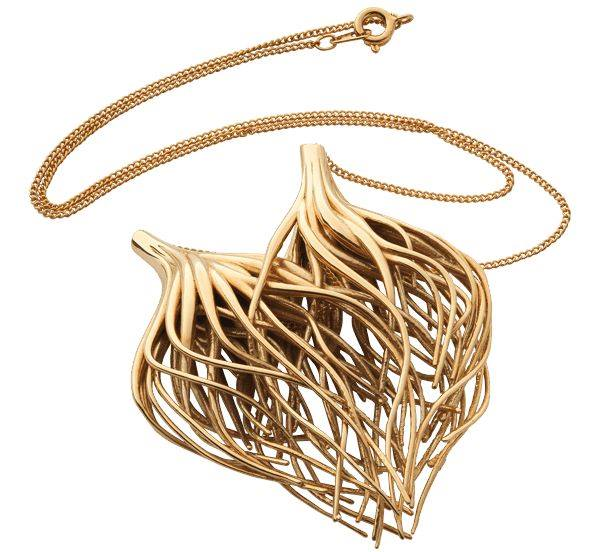
\includegraphics[height=3.6cm]{introduction/jewelry.jpg}
      }
      \subfloat[3D-printed Prohstetics]{
        \label{fig:expertise-prosthetic}
        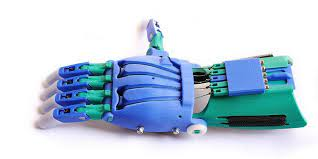
\includegraphics[height=3.6cm]{introduction/enable.jpeg}
      }
      \label{}

      \caption{Although current digital fabrication devices can be used to
        create a variety of objects, like jewelry (Figure
        \ref{fig:expertise-jewelry}) or prosthetics (Figure
        \ref{fig:expertise-prosthetic}) designers require domain expertise to
        create this objects.}
    \end{figure}

    The second issue relates to the expertise required to construct usable
    objects. While current personal fabrication equipment is able to produce a
    variety of interesting objects from prosthetic arms for children (Figure
    \ref{fig:expertise-prosthetic}) to intricate jewelry pieces (Figure
    \ref{fig:expertise-jewelry}), the construction of these objects require
    ample domain knowledge that consumers might not possess.  This leaves very
    limited options for low-entry uses for fabrication devices.

  \section{Towards On-Demand Fabrication of Interactive Devices} \label{sec:on-demand}
    Despite the utility of custom-made three-dimensional shapes, recent work has
    highlighted that ``everyday makers'' are most interested in fabricating
    objects they can interact with~\cite{Shewbridge:2014}. Inspired by these
    findings, and the personal fabrication ideal described in Section
    \ref{sec:fab-revolution}, this thesis explores a potential future where
    digital fabrication equipment not only enables the construction of custom
    three-dimensional shapes, but of tangible devices as well.

    The creation of these tangible devices should be as natural and automatic as
    possible. Similarly to today's document creation pipeline, where once the
    document is constructed in a word processing software, and sent to the
    desktop printer there are no further actions to carried out, so should be
    the creation process of tangible devices. Designers should be able to model
    their desired device using a CAD software suite, send this design to a
    personal fabrication machine, and once printed, no post-print activities
    should be necessary to materialize the device.

    \subsection{Challenges}
      The concept of constructing interactive devices using digital fabrication
      equipment is not new. A multitude of research endeavors in the
      Human-Computer Interaction (HCI) community have explored techniques to
      fabricate interactive devices using 3D-printers or other digital
      fabrication equipment~\cite{Ballagas:2018}. However, despite these
      advances, the introduced techniques have yet to escape the research
      laboratories and move on into the masses. This is due to two main factors:

      \subsubsection*{Convoluted Fabrication Pipelines}
        A paramount research challenge researchers need to resolve is the
        democratization of techniques. Revisiting the paper document metaphor,
        when the same document is printed in different types of 2D printers, the
        outcome is the same. So it should be when constructing interactive
        devices: the method of construction should not affect the capability of
        the device. Additionally, we should strive to automate the construction
        process as much as possible, opting to use accessible fabrication
        machines and devices over manual labor. We should also avoid using
        non-accessible materials.

      \subsubsection*{Complex Post-Print Activities}
        An additional challenge is the removal of complex post-print activities.
        Current fabrication pipelines for the construction of interactive
        devices rely on convoluted post-print activities in order to fabricate
        these devices. These post-print activities can take the shape of
        assembly of circuits, printed parts, complex removal of support
        material, or calibration of per-object, or per-user machine learning
        models. This means that in order for non-experts to construct tangible
        devices they must be well-versed in electronics, programming, and
        mechanics---limiting the adoption of the proposed techniques.
      
    \subsection{\papf}
      As a way towards the potential future of on-demand fabrication of
      interactive devices described in Section \ref{sec:on-demand}, this thesis
      introduces \papf: a digital fabrication paradigm where interactive objects
      are printed instead of assembled. \pap fabrication techniques construct
      devices that are immediately usable after fabrication, meaning there is no
      assembly of parts, circuits, or calibration of machine learning models
      needed. Additionally, \pap techniques, are constructable using
      off-the-shelf fabrication equipment and materials.

      The concept of \papf directly addresses the shortcomings of the personal
      fabrication revolution described in Section \ref{sec:broken-promises}.
      First in increases the versatility of off-the-shelf fabrication materials
      and printers. All \papf should be able to be instantiated using
      consumer-grade fabrication equipment and materials. Second, \pap
      techniques should not require any post-print activities or domain-specific
      knowledge (e.g., programming, electronics) to be enabled. Additionally,
      they must provide a design environment to streamline the modeling of
      tangible devices by non-expert designers. These two factors increase the
      target audience of these techniques.

      \subsubsection*{Contributions of this Thesis}
        This thesis focuses on the easy construction of tangible devices without
        requiring significant post-fabrication activities (e.g., assembly of
        parts, circuits, calibration of machine learning models), or specialized
        fabrication pipelines. The work encompassed in this document presents
        techniques for constructing tangible devices that can sense, process,
        and provide output to user's interactions. I achieve this by embedding
        custom geometries in the interior of three-dimensional models that
        leverage well-studied physical phenomena such as fluid dynamics, or
        acoustic resonance.
        
        An overarching theme of this work is \emph{air}. All of the work
        presented in this thesis is powered by air, being from a constant,
        pressurized air source (Chapters \ref{ch:airtouch}, \ref{ch:morphees},
        and \ref{ch:airlogic}), or from the user's lungs (Chapter
        \ref{ch:blowhole}). The use of air as a medium to enable the
        construction of interactive devices was motivated by two factors. First,
        air and fluid behaviors have been extensively explored in physics, which
        gives us a ample understanding how air behaves in a variety of
        situations, and which ones of these lend themselves to digital
        fabrication pipelines. Second, thanks to the broad understanding of
        fluid behavior, we can employ these concepts to construct pre-trained
        machine learning models, or use their respective mathematical equations,
        to identify user's interactions.
        
        The papers that make up this thesis explicitly address the challenges
        described above. First, the interactive devices constructed using the
        proposed techniques are printed in commodity 3D printers as a single
        structure, requiring no post-print assemblies of parts. Second, because
        they embed custom interior structures in the interior of the augmented
        designs, and leverage well-studied physical phenomena to enable
        interactions, they require no electronics to sense, process, or provide
        output to user's interactions. Third, as an additional benefit of
        leveraging well-studied physical phenomena to enable interactions, these
        devices employ mathematical models, or pre-trained machine learning
        models, requiring no per-object, or per-user calibration. A summary of
        the individual contributions of the papers that comprise this document
        can be found below:

        \textsc{\at} extends the possibilities of pneumatic sensing on
        fabricated objects by enabling sensing users interactions not only on
        soft objects, but in rigid ones as well. \emph{\at} is based on basic
        principles of fluid dynamics that relate pressure to discharge area:
        when there is a change in the discharge area of a system, the pressure
        will vary in return. Objects augmented with \emph{\at} can sense touch
        interactions in up to 12 individual locations, and are printed as a
        single structure. These objects are fabricated as a single structure
        without requiring any assembly of parts or circuits. Additionally, they
        make use of pre-trained machine learning models, so no per-object or
        per-user calibration is necessary.
        
        \textsc{\bh} continues to explore techniques for enabling sensing of
        user's interactions on 3D-printed objects by addressing one of
        \emph{\at's} principals shortcomings: the need for a constant air source
        and barometric pressure sensors. Based on the principle of acoustic
        resonance, \emph{\bh} embeds resonant cavities in the interior of the
        model that, when gently blown on, emit an identifiable sound.
        Interactive devices constructed using \emph{\bh} are fabricated as a
        single structure using commercially-available printers and materials,
        and make use of a mathematical model to identify blow locations based on
        the frequency of the generated sound.

        Switching gears to computing, \textsc{AirLogic} aims to answer the
        question ``how can we 3D-print devices that can think?'' Inspired by
        research from the Cold War era, I developed a series of widgets that can not
        only sense user's interactions, and provide output to them, but also
        compute simple logic operations (e.g., \texttt{AND, OR, NOT}, and
        \texttt{XOR}).

        Last, with \textsc{MorpheesPlug} I explore the construction of devices
        that can provide physical output. This work was inspired by recent
        research on shape-changing interfaces, where physical interfaces change
        their shape depending on their intended use. We approached this concept
        from a fabrication standpoint, creating a set of pneumatically-actuated
        widgets that can represent a variety of changes in shape. These widgets
        are fabricated as a single structure, using off-the-shelf printers and
        materials.